% !TeX root = RJwrapper.tex
\title{GCalignR. An R package for aligning Gas-Chromatography data}
\author{by Meinolf Ottensmann, Martin A. Stoffel, Joseph I. Hoffman}

\maketitle

\abstract{%
This is just a placeholder for 150 words in the abstract This is just a
placeholder for 150 words in the abstract This is just a placeholder for
150 words in the abstract This is just a placeholder for 150 words in
the abstract This is just a placeholder for 150 words in the abstract
This is just a placeholder for 150 words in the abstract This is just a
placeholder for 150 words in the abstract This is just a placeholder for
150 words in the abstract This is just a placeholder for 150 words in
the abstract This is just a placeholder for 150 words in the abstract
This is just a placeholder for 150 words in the abstract This is just a
placeholder for 150 words in the abstract This is just a placeholder for
150 words in the abstract
}

\section{Introduction}

Chemical cues are arguably the most common mode of communication among
animals \citep{Wyatt.2014}. By exploring broad patterns in complex
chemical signatures, researchers make inferences on kinship
\citep{Krause.2012, Stoffel.2015}, genetic diversity
\citep{Charpentier.2010, Leclaire.2012}, sexual maturation
\citep{Caspers.2011} or species discrimination
\citep{Meulemeester.2011}. One of the most common instruments to
quantify the chemical composition of samples is gas-chromatography, a
fast high-throughput method to detect individual chemicals and their
abundances \citep{McNair.2011}, while the additional implementation of
mass-spectrometry (GC-MS) allows to identify specific substances
\citep{Caspers.2011}. \par
However, before similarity patterns across can be analysed, it is
essential to align compounds among samples, thereby accounting for
drifts in the retention times of peaks caused by subtle, random and
often unavoidable variations of the chromatography machine parameters
\citep{Pierce.2005}. Many studies rely on manual alignment rather than
(semi-)automated algorithms (citations necessary), but this approach
bears three severe drawbacks: (1) In large scale studies this task
becomes increasingly time consuming task and is impracticable. (2)
Humans are prone to detect patterns in noise which is why the researcher
may bias the alignment due to subjective experience and expectations.
(3) The data analytic pipeline from the raw gas-chromatography data to
the results of the statistical analysis is not reproducible. (citations
for the first two points necessary) Several alignment algorithms have
been proposed to overcome these issues, but these focus nearly
exclusively on GC-MS data \citep{Pierce.2005, Robinson.2007,Jiang.2013}
and only some a easily accessible as web-based tools
\citep{Hoffmann.2009, Wang.2010} or independent software
\citep{Dellicour.2013}. \par
Here, we introduce \pkg{GCalignR}, a package that implements a simple
and fast algorithm to align peaks from GC data and evaluate the
resulting alignment using two data sets. \pkg{GCalignR} was specifically
developed as a tool for pre-processing GC data from animal skin and
preen glands prior to subsequent statistical analysis. In brief, the
algorithm consists of two main steps: (1) Systematic shifts of
chromatograms are corrected by applying appropriate linear shifts to
whole chromatograms based on a single reference. (2) Retention times of
individual peaks are grouped iteratively together with homologous peaks
of other samples and aligned within the same row in a retention time
matrix . The quality of this grouping procedure can be adjusted to
specific datasets through three parameters that are described in detail
below. Among several optional processing steps, the package allows to
remove peaks belonging to contaminations, which are identified due to
their presence in control samples. For an easy interpretation of the
quality of an alignment we implemented several ways to plot the outcome
(You can change this to something more specific). Furthermore, we
demonstrate a complete workflow from chemical raw data to multivariate
analyses with the popular and widely used
\href{https://cran.r-project.org/web/packages/vegan/index.html}{\CRANpkg{vegan}}
\citep{Oksanen.2016} package. This allows the integration of the full
analysis into \strong{RMarkdown} documents \citep{Allaire.2016} in order
to meet the standards of reproducibility \citep{Peng.2011}.

\section{The Package}

\pkg{GCalignR} consists of functions that allow the alignment of peaks
from GC and GC-MS data based on retention times. The main aim of the
package is to provide a simple tool that guides the user through the
unbiased alignment of large data sets prior to hypothesis-testing of the
multivariate data \citep{Anderson.2001}. We summarise the underlying
algorithm and workflow (figure \ref{figure:workflow}) below and refer to
the vignette that can be assessed via
\code{browseVignettes('GCalignR')}.

\begin{figure}[htbp]
  \centering
  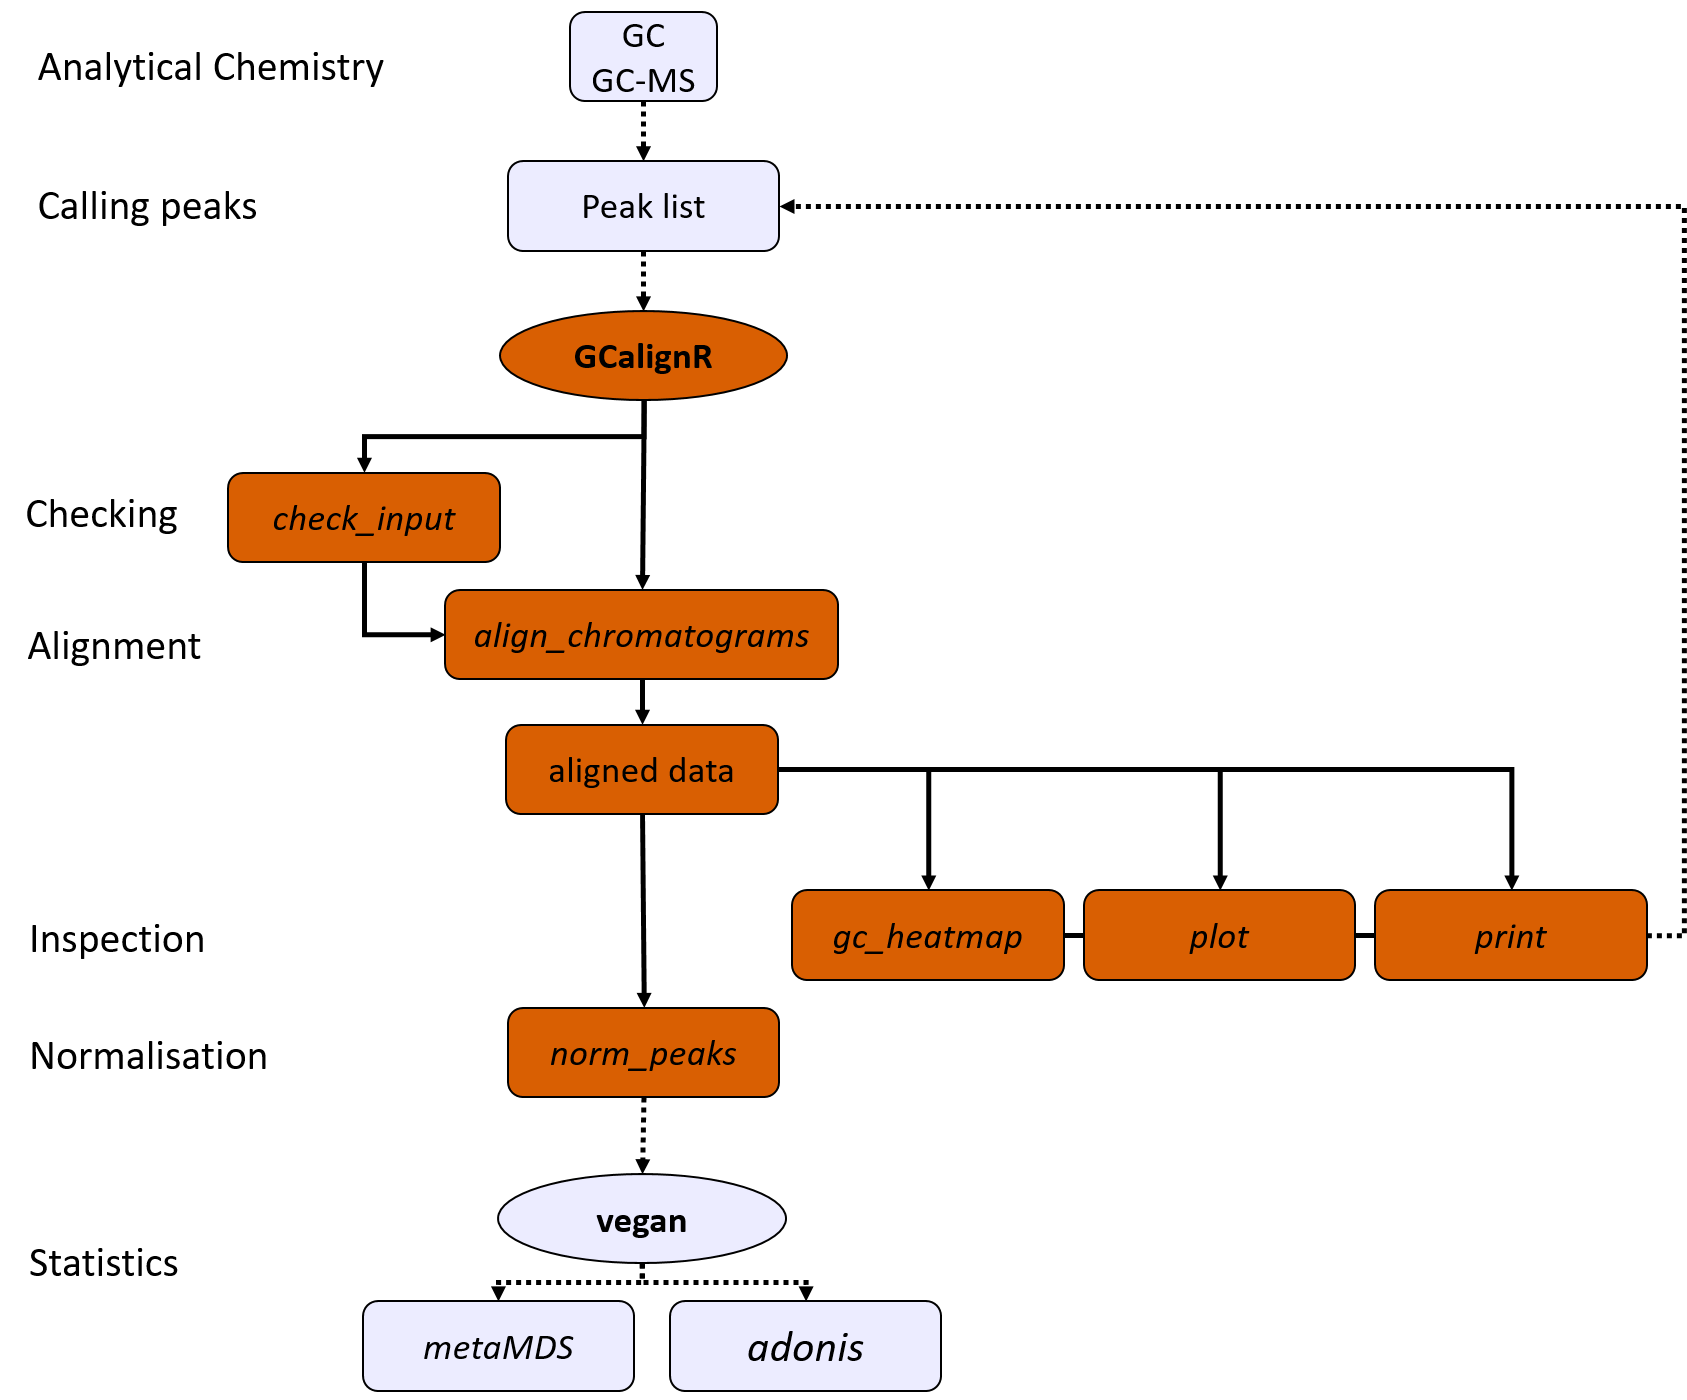
\includegraphics[width=13cm]{figures/workflow}
  \caption{\pkg{GCalignR} workflow. In addition to the alignment of substances across samples, the package provides functions for checking and inspecting the data. The aligned data is ready to use for analyses in conjunction with other packages. Each function is explained within the text.}
  \label{figure:workflow}
\end{figure}

\subsection{Example dataset}

For demonstration purposes \pkg{GCalignR} includes data of chemical
signatures that were obtained by sampling the skin of 82 Antarctic fur
seals \textit{Arctocephalus gazella}. It was previously shown that these
signatures encode the membership to a breeding colony
\cite{Stoffel.2015}. These data are available as a \emph{list} with
individual samples included as a \emph{data.frame}. Two variables are
available that represent the required retention time (``time'') and
concentration or peak abundance (``area'') within a sample.

\begin{Schunk}
\begin{Sinput}
library(GCalignR)
# Seal scent data
data("peak_data") 
# Data is organized in one list of data frames
str(peak_data[1:2]) 
\end{Sinput}
\begin{Soutput}
#> List of 2
#>  $ C3:'data.frame':  217 obs. of  2 variables:
#>   ..$ time: num [1:217] 4.53 4.55 4.62 4.68 4.71 4.79 4.83 4.87 5.01 5.14 ...
#>   ..$ area: num [1:217] 3331224 1462381 4834211 7754401 1267617 ...
#>  $ C2:'data.frame':  217 obs. of  2 variables:
#>   ..$ time: num [1:217] 4.52 4.55 4.57 4.67 4.69 4.73 4.75 4.8 4.83 4.85 ...
#>   ..$ area: num [1:217] 2695110 5926253 10406833 6805905 1672849 ...
\end{Soutput}
\end{Schunk}

The package provides the function \textbf{check\_input} to test the
input file for typical formatting errors and incomplete data. We
encourage to use unique names for samples that consist only of letters,
numbers and underscores. If the data fails the test, indicative warnings
are returned which guide in correcting the errors. Prior to the start of
any alignment this function is used internally.

\begin{Schunk}
\begin{Sinput}
check_input(peak_data)
\end{Sinput}
\begin{Soutput}
#> All checks passed!
#> Ready for processing with align_chromatograms
\end{Soutput}
\end{Schunk}\subsection{Aligning substances among samples}

The alignment procedure is divided into five steps (figure
\ref{figure:algorithm}). All steps are executed by the main function
\emph{align\_chromatograms} and will be explained in in the next
sections. \subsubsection{Linear adjustments of chromatograms} At first,
chromatograms are linearly shifted with respect to a reference sample to
account for systematic shifts in retention times among homologous
chemicals shared by samples. Therefore, same small linear adjustments
are applied to the entire set of peaks in a chromatogram (figure
\ref{figure:algorithm} A), such that the number of peaks that are shared
between the sample and the reference at a given threshold (i.e.~0.6
seconds) is maximised.The parameter \emph{max\_linear\_shift} defines
the maximum temporal range of linear shifts that are considered by the
program. \newline
Note: This method relies on the occurrence of substances that are shared
among most substances to produce efficient adjustments. If those are
absent, it is unlikely to find a suitable shift and chromatograms remain
untransformed. \par
A reference may be selected automatically by searching for the sample
with the highest average similarity to all other samples based on the
number of shared peaks prior to alignment. Alternatively, a chromatogram
may be included that contains peaks of an internal standard which peaks
are \textit{a-priori} known to occur in all samples. In this case, the
sample is named \code{"reference"} and will be removed after the
alignment was conducted.

\newpage

\begin{figure}[htbp]
  \centering
  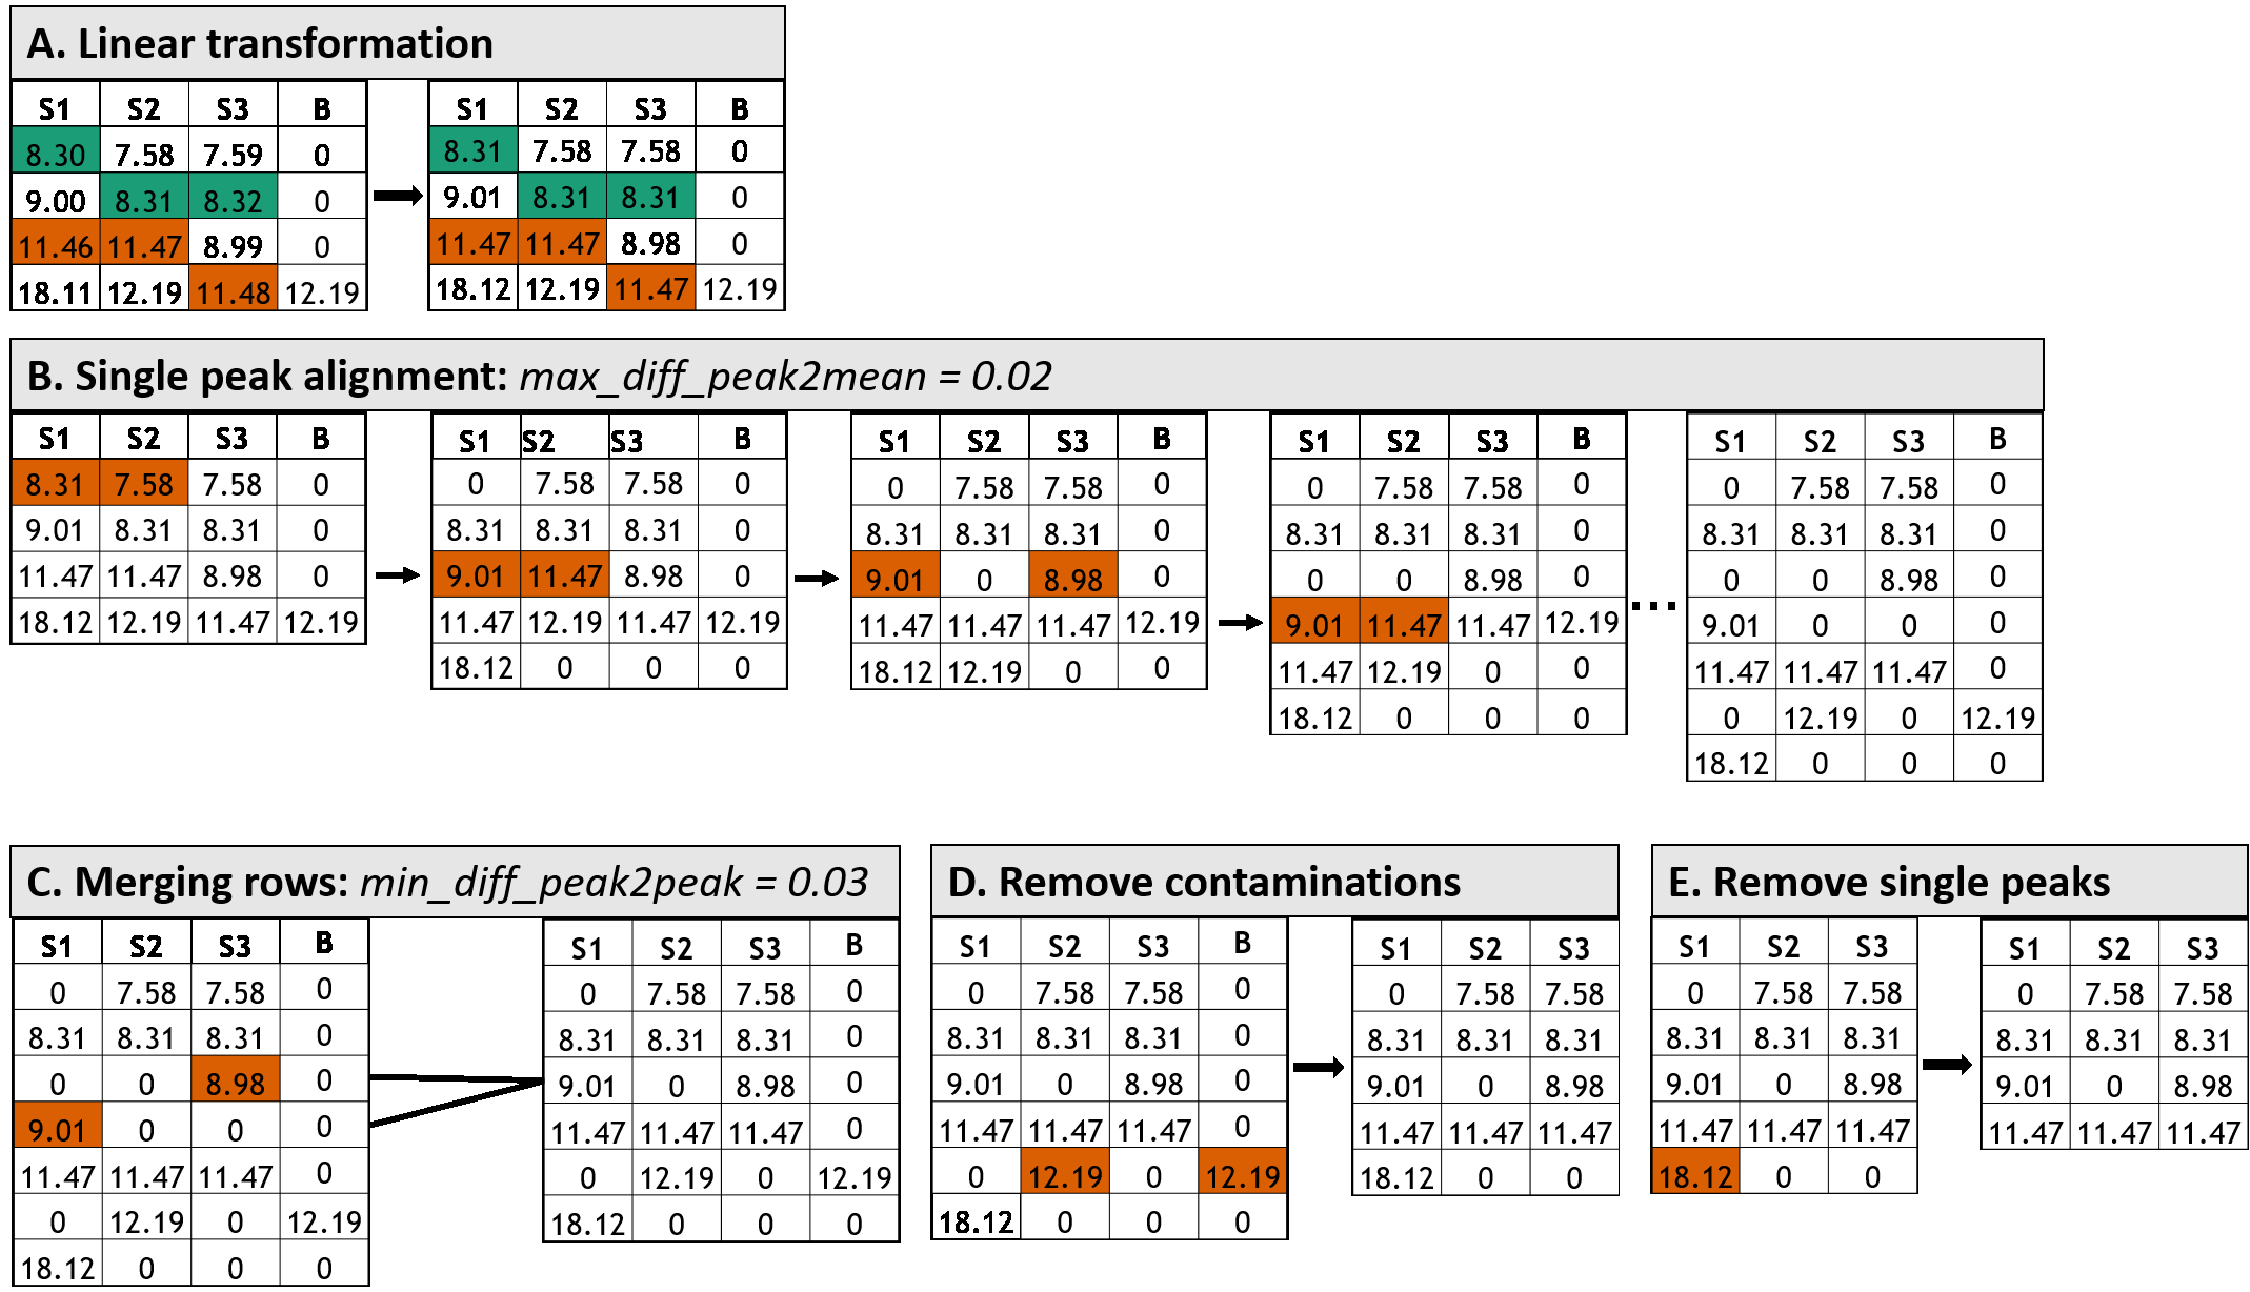
\includegraphics[width=13cm]{figures/algorithm}
  \caption{Overview of the algorithm performed by GCalignR. Rows of matrices correspond to substances, columns are samples. Zeros indicate absence of peaks and are ignored in calculations. \strong{A}. Chromatograms are linearly shifted with respect to a reference (S2). Strong{B}. From left to right the first four steps from the input matrix to the final alignment are shown. Peaks are aligned row by row. Initially, always the second sample is compared to the first. Then the next sample is compared to all samples in previous columns until the last column is reached. Coloured cells represent conflicting retention times using \code{max_peak2mean = 0.02}. \strong{C}. After all peaks have been aligned, rows are merged depending on \code{min_peak2peak}, which defines the minimum difference that is expected between substances. If merging does not result in the loss of any data, rows are merged. \strong{D}. If specified, all peaks found in one or more blanks (negative control) are removed as well as the blank itself. \strong{E}. Unique peaks which are present in only a single individual are not of interest for similarity analyses and can be removed as well.}
  \label{figure:algorithm}
\end{figure}

\subsubsection{Peak alignment}

The core of the alignment procedure is based on clustering of individual
peaks among samples. This is performed by examining retention times
within single rows, where samples are compared consecutively with all
previous samples starting with the second column (figure
\ref{figure:algorithm} B):\par

\begin{equation}
rt_{m} > \left(\frac{\sum_{i=1}^{m-1}rt_{i}}{m-1}\right) + max_peak2mean
\end{equation}

If the examined peak is moved into the next row, whereas all previous
samples are moved \par

\begin{equation}
rt_{m} < \left(\frac{\sum_{i=1}^{m-1}rt_{i}}{m-1}\right) - max_peak2mean
\end{equation}

with \textit{rt} = retention time; \textit{m} = current column and
\textit{max_peak2mean} defining the maximal deviation of the mean
retention time. \newline By considering the mean retention time among
all previous samples the algorithm accounts for substance specific
variations, such that less variable retention times are treated more
stringent than chemicals exhibiting higher variability. Once the last
retention time of a row was evaluated the whole procedure is repeated
with the next row until the end of the retention time matrix was
reached. \subsubsection{Merging} Afterwards, rows with similar mean
retention times are assessed for redundancy (figure
\ref{figure:algorithm} C), which applies whenever a merging does not
cause any loss of any information (i.e.~no sample exists that contains
substances in both rows). The similarity threshold is given by
\textit{min_peak2peak} defining the minimal difference between peaks
that is expected. \par 

\subsection{Post processing}

After aligning peaks the package offers several optional post processing
steps that allow to cleanup the data.
\subsubsection{Removing contaminations} Among other sources, residues of
unwanted chemical substances in the gas chromtography column or within
reagents used in the laboratory have the potential to contaminate
chemical samples. To get rid of these substances it is avdisable to
include negative controls that have been treated in the very same way as
the acutal samples but have not been used to sample and individual´s
skin for instance. Within \code{align_chromatograms} those samples can
be included in the data set as \textit{blanks}. Blanks are treated as
normal samples during all alignment steps and are afterwards used to
identify contaminants with are in turn removed from the data as well as
the negative controls itself. \subsubsection{Removing single peaks}
Sometimes substances occur that are only found within a single sample.
For comparative approaches that calculate simmilarity mattrices these
substances are not informative and can be removed from the data for
reasons of simplicity. \pkg{GCalignR} allows to do so using the logical
\code{delete_single_peak}. \subsubsection{Normalisation} Many
multivariate analysis techniques, like those available in \pkg{vegan},
require a data frame of independent variables as input format. Moreover
is generally advisable to normalise abundancies prior to statistical
analysis to correct for variations in the total concentration of
samples. This is utilised in \pkg{GCalignR} function
\code{normalise_peaks} which normalises peak abundancies by calculating
realtive abundancies for each sample.

\section{Workflow}

Here, we demonstrate the typical workflow using our seal data. All
alignment steps that have been described above are implemented within
the function \texttt{align\_chromatograms}. A list of all parameters and
their description can be assessed from the documentation in the helpfile
by typing \texttt{?align\_chromatograms}. As it is outlined in

\begin{Schunk}
\begin{Sinput}
seal_aligned <- align_chromatograms(data = peak_data,
                    conc_col_name = "area",
                    max_diff_peak2mean = 0.03,
                    min_diff_peak2peak = 0.05,
                    max_linear_shift = 0.05,
                    rt_col_name = "time",
                    delete_single_peak = TRUE,
                    blanks = c("C2","C3")) # negativ controls
\end{Sinput}
\begin{Soutput}
#> All checks passed!
#> Ready for processing with align_chromatograms
#> Run GCalignR
#> Start: 12:25:58
#> 
#> Data for 84 samples loaded.
#> A reference was not specified. Hence, 'P31' was selected on the basis of highest
#> average similarity to all samples (score = 37).
#> Start Linear Transformation with "P31" as a reference ... Done
#> Start Alignment of Peaks ...  This might take a while!
#> Iteration 1 out of 1  ... 
#> Merged Redundant Peaks
#> Peak Alignment Done 
#> 
#> Blank Peaks deleted & Blanks removed
#> 
#> Single Peaks deleted: 61 have been removed
#> 
#> Alignment was successful!
#> Time: 12:43:48
\end{Soutput}
\end{Schunk}

Now, we can inspect the results by retrieving summaries of the alignment
process. The printing method summarises the function call including
defaults that have not been explicitly specified during the function
call. We also get the relevant information to retrace every step in the
alignment:

\begin{Schunk}
\begin{Sinput}
print(seal_aligned)
\end{Sinput}
\begin{Soutput}
#>   Summary of Peak Alignment running align_chromatograms from package GCalignR
#>   Input: peak_data   Start:  2017-01-12 12:25:58     Finished:  2017-01-12 12:43:48 
#> 
#> Call:
#>   GCalignR::align_chromatograms(data=peak_data, conc_col_name=area,
#>   rt_col_name=time, max_linear_shift=0.05, max_diff_peak2mean=0.03,
#>   min_diff_peak2peak=0.05, blanks=(C2, C3), delete_single_peak=TRUE, sep=\t,
#>   rt_cutoff_low=NULL, rt_cutoff_high=NULL, reference=NULL, iterations=1)
#> 
#> Summary of scored substances:
#> 
#>     Peaks In_Blanks  Singular  Retained 
#>       480       169        61       250 
#> 
#>   In total 480 substances were identified among all samples. NA substances were
#>   present in blanks. The corresponding peaks as well as the blanks were removed
#>   from the data set. 61 substances were present in just one single sample and were
#>   removed. 250 substances are retained after all filtering steps.
#> 
#> Sample Overview  The following 84 Samples were aligned to the reference 'P31':
#>   M2, M3, M4, M5, M6, M7, M8, M9, M10, M12, M14, M15, M16, M17, M18, M19, M20,
#>   M21, M23, M24, M25, M26, M27, M28, M29, M30, M31, M33, M35, M36, M37, M38, M39,
#>   M40, M41, M43, M44, M45, M46, M47, M48, P2, P3, P4, P5, P6, P7, P8, P9, P10,
#>   P12, P14, P15, P16, P17, P18, P19, P20, P21, P23, P24, P25, P26, P27, P28, P29,
#>   P30, P31, P33, P35, P36, P37, P38, P39, P40, P41, P43, P44, P45, P46, P47, P48
#> 
#> For further details:
#>   Type 'gc_heatmap(seal_aligned)' to retrieve a heatmap for the alignment accuracy
#>   Type 'plot(seal_aligned)' to retrieve further diagnostic plots
\end{Soutput}
\end{Schunk}

The quality of an alignment will depend on sensible parameters that
facilitate the (i) correction of linear shifts that might fall in a
larger range with increasing sample size and (ii) and the variability of
retention times. Optimally, linear shifts do not exhaust the range given
by \texttt{max\_linear\_shift} completely, which would in turn indicate
that not all uncertainties haven been fully compensated for. This can be
assessed by some diagnostic plots:

\begin{Schunk}
\begin{Sinput}
plot(seal_aligned)
\end{Sinput}

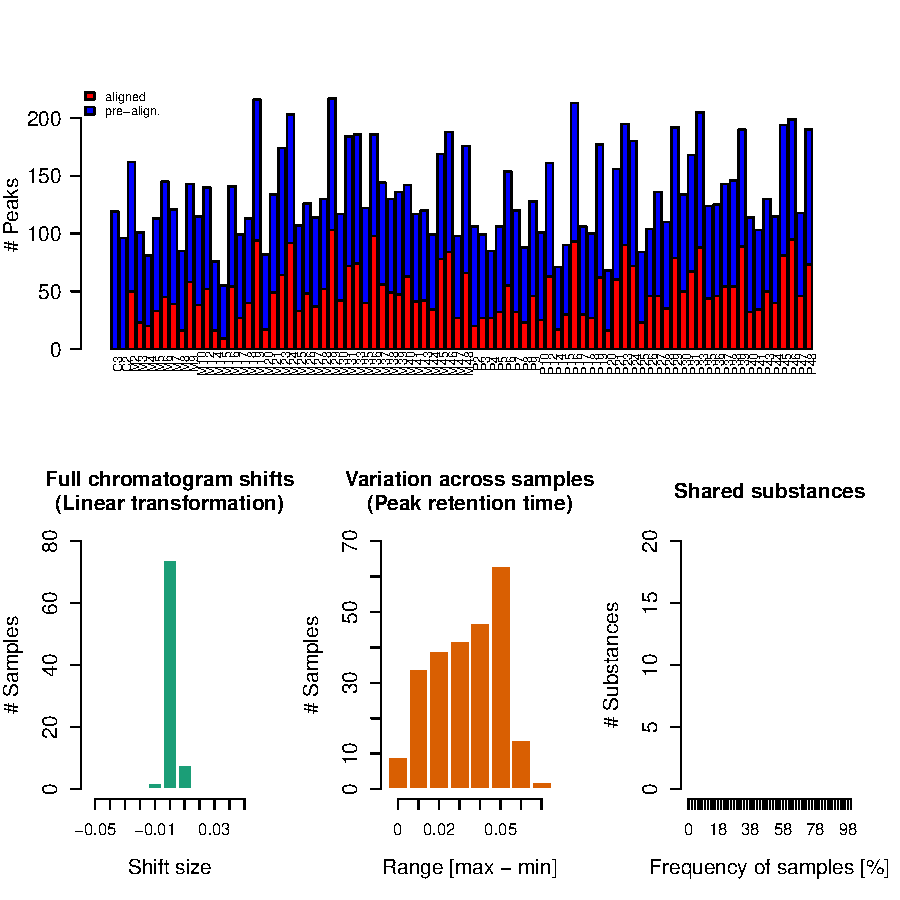
\includegraphics{ottensmann-stoffel-hoffman_files/figure-latex/unnamed-chunk-5-1} \begin{Sinput}
gc_heatmap(seal_aligned,type = "continuous", substance_subset = 1:25, samples_subset = 1:25)
\end{Sinput}

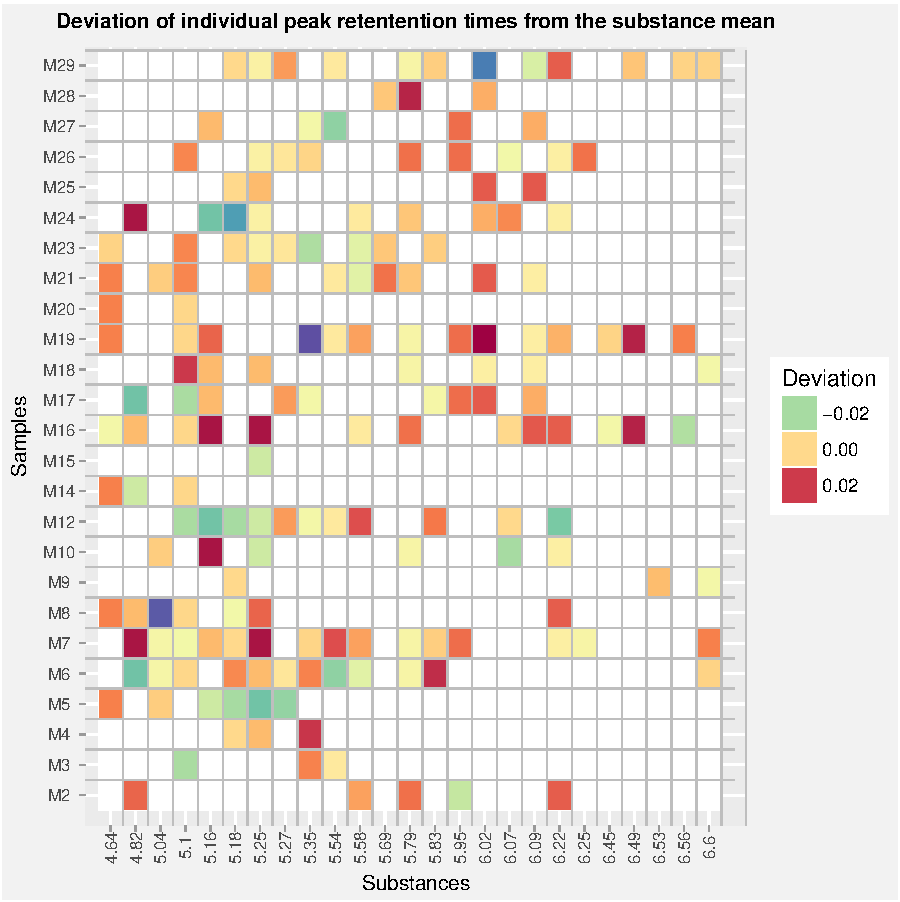
\includegraphics{ottensmann-stoffel-hoffman_files/figure-latex/unnamed-chunk-5-2} \end{Schunk}

\bibliography{ottensmann-stoffel-hoffman}

\address{%
Meinolf Ottensmann\\
Department of Animal Behaviour\\
Bielefeld University\\ Morgenbreede 45\\ 33615 Bielefeld\\
}
\href{mailto:Meinolf.Ottensmann@web.de}{\nolinkurl{Meinolf.Ottensmann@web.de}}

\address{%
Martin A. Stoffel\\
Department of Animal Behaviour\\
Bielefeld University\\ Morgenbreede 45\\ 33615 Bielefeld\\
}
\href{mailto:Martin.Adam.Stoffel@gmail.com}{\nolinkurl{Martin.Adam.Stoffel@gmail.com}}

\address{%
Joseph I. Hoffman\\
Department of Animal Behaviour\\
Bielefeld University\\ Morgenbreede 45\\ 33615 Bielefeld\\
}
\href{mailto:j_i_hoffman@hotmail.com}{\nolinkurl{j\_i\_hoffman@hotmail.com}}

